\chapter{Vorgehen}
Model der Machbarkeitsstudie ausmessen und Entwicklungspunkte definieren.

\section{Inbetriebnahme des Modells der Machbarkeitsstudie}
Mit der in der Projektarbeit entwickelten Harvesterschaltung kann per Bluetooth Smart auf dem Android-Endgerät die Geschwindigkeit ausgegeben werden.
Bei der Inbetriebnahme zeigten sich folgende Grenzen im gegebenen Modell:

\begin{enumerate}
    \item Zu hoher Kondensator vor Energiemanagmenetschaltung gefährdet deren Stabilität
    \item Konfiguration auf Energiemanagementboard sind nicht auf EnergieHarvesterSchaltung angepasst
    \item ???
\end{enumerate}



\subsubsection{Kapazität für Harvesting-Schaltung verbessern}
In der Machbarkeitsstudie ist nach dem Gleichrichter ein Kondensator von 470 uF nachgeschaltet. Dieser glättet die Spannungspulse nach dem Gleichrichter zu einer DC-ähnlichen Spannung mit Rippeln.

Mit einem Kondensator von 470 uF wird die Ausgangsspannung der Harvesterspannung fast rippelfrei. Die Rippelspannung beträgt 3.2 mV (siehe Abbildung \ref{kond470uF}).
\begin{figure}
    \includegraphics[bb = 0 0 100 100]{3Vorgehen/imag/470uF.PNG}
    \caption{Rippelspannung bei Glättung mit 470 uF Kondensator}\label{kond470uF} 
\end{figure}

Gemäss Ives \textbf{XXXXXX} von EMMicroelectronics sollten Kondensatoren der Harvesterschaltung im Bereich von 47 uF liegen, sodass die Energiemanagementschaltung ordnungsgemäss funktioniert.  

Aus diesem Grund wird die Rippelspannung am Ausgangs der Harvesterschaltung mit kleineren Kondensatoren gemessen. Das Messprotokoll befindet sich im Anhang.

\subsubsection*{Messaufbau}
In der gegebenen Harvesterschaltung wird am Kondensator die Spannung mit einem Kathodenstrahloszilloskop (KO) gemesssen. Ausgehend vom bestehenden Kondensator (470 uF), werden danach Elektrolytkondensatoren (Elko) mit den Werten 100 uF, 47 uF und 10 uF gemessen.

\begin{figure}
    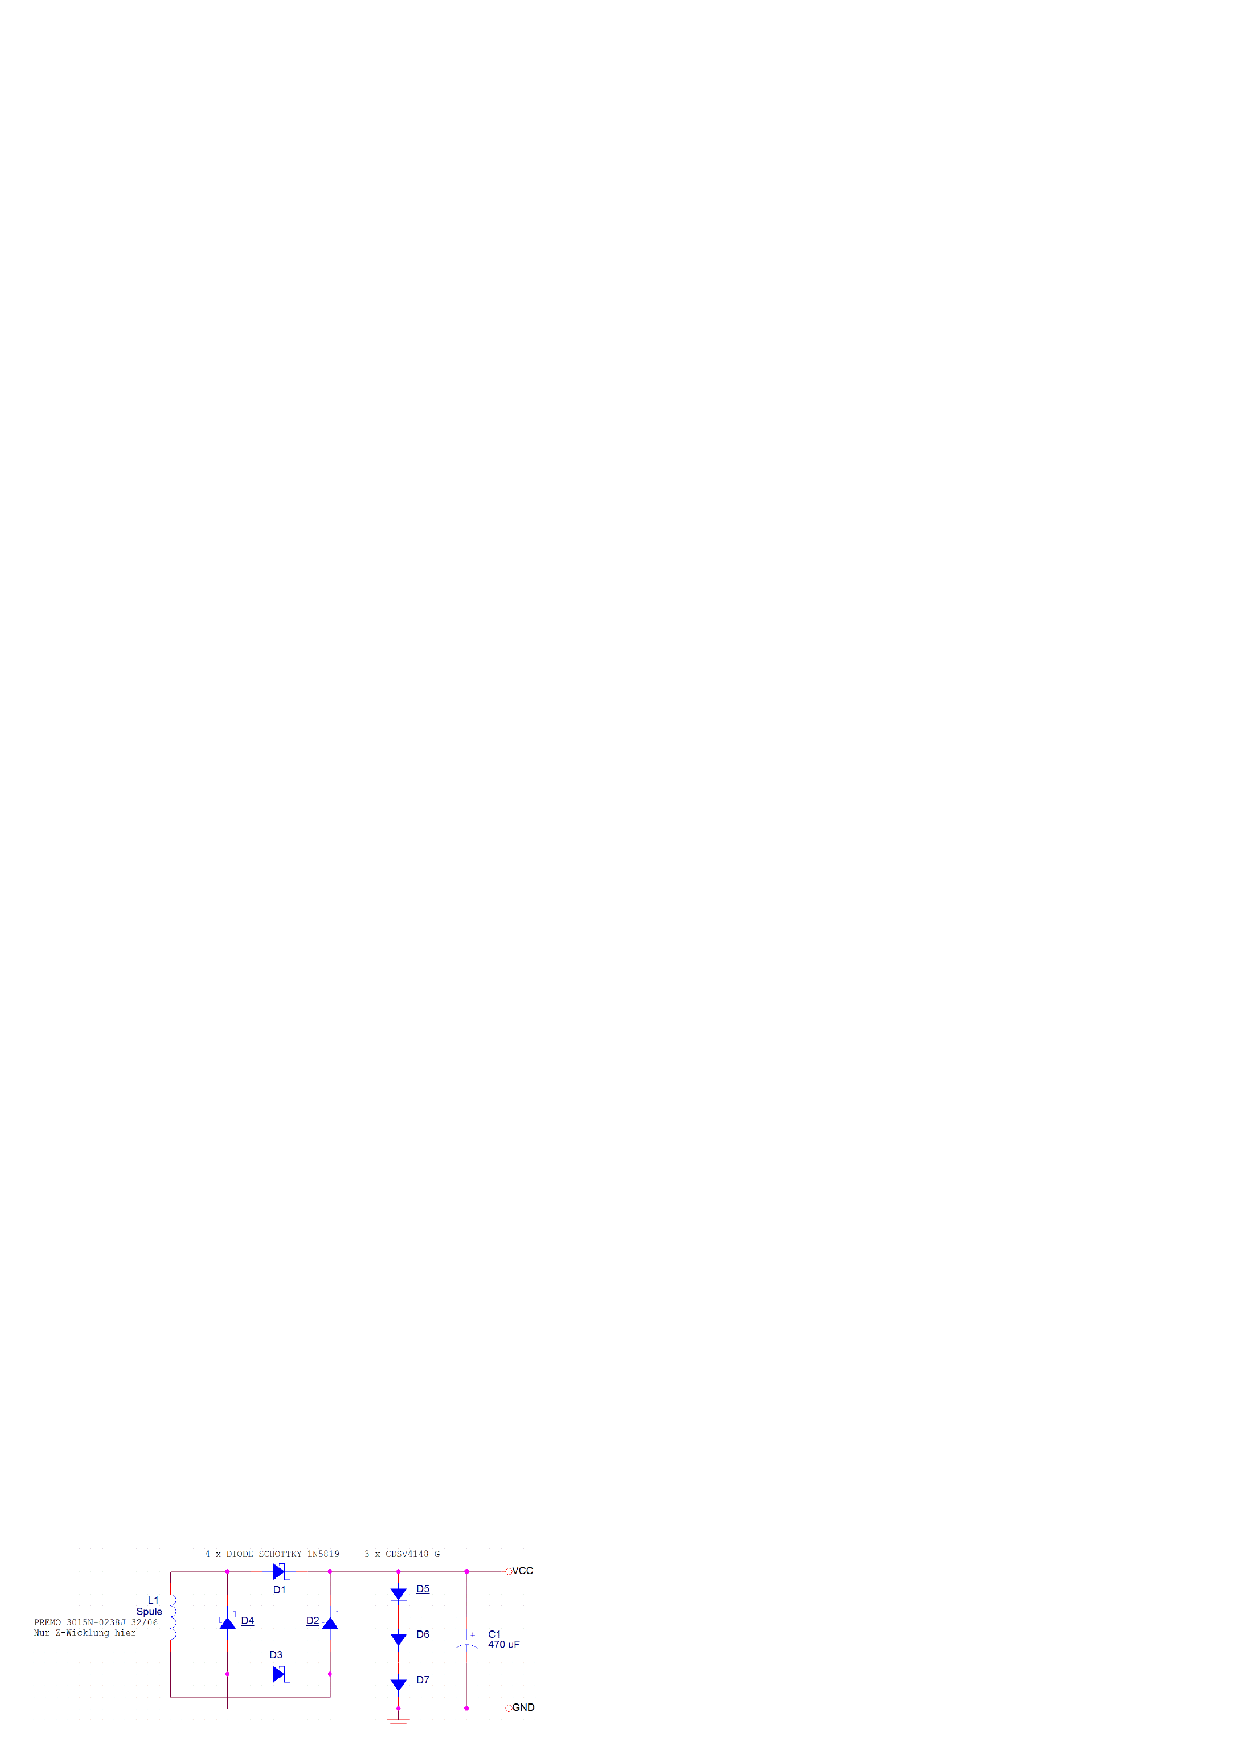
\includegraphics[bb = 0 0 100 100]{3Vorgehen/imag/messschaltungHarvesterschaltung.jpg}
    \caption{Messschaltung}
\end{figure}

\subsubsection*{Resultat}

Die Rippelspannung erhöht sich wie erwartet. Vpp beträgt bei 100 uF \textbf{xx} mV, bei 47 uF 28.8 mV (siehe Abbildung \ref{kond47uF}) und bei 10 uF 320 mV (Abbildung \ref{kond10uF}).
 
\begin{figure}
    \includegraphics[bb = 0 0 100 100]{3Vorgehen/imag/10uF.PNG}
    \caption{Rippelspannung mit 10 uF Kondensator}\label{kond10uF} 
\end{figure}

\begin{figure}
\includegraphics[bb = 0 0 100 100]{3Vorgehen/imag/47uF.PNG}
\caption{Rippelspannung mit 47 uFKondensator}\label{kond47uF} 
\end{figure}


\subsubsection{Messungen Energy Management Board}

\begin{figure}
\includegraphics[bb = 0 0 100 100]{3Vorgehen/imag/messungPA.png}
\caption{Rippelspannung mit 47 uFKondensator}
\end{figure}
Es zeigt sich, dass der LTS nicht geladen wird . Und es zeigt sich, dass das EM-Board nicht zu regulieren beginnt.








\pagebreak
\subsubsection{Messungen Sensortag}
Ziel: Energieverbrauch kennen.

Unterschied zwischen dem Programmierten Sensortag des Prototypen und dem neuen Sensortag.




\section{Layout Print}

\section{Kommunikation Bluetooth Low Energy}

\section{Energieoptimierung}



\section{Applikationsentwicklung}

\section{Option 1}






